\prob
{
    Prove that the next matrix is totally unimodular.
    \begin{center}
        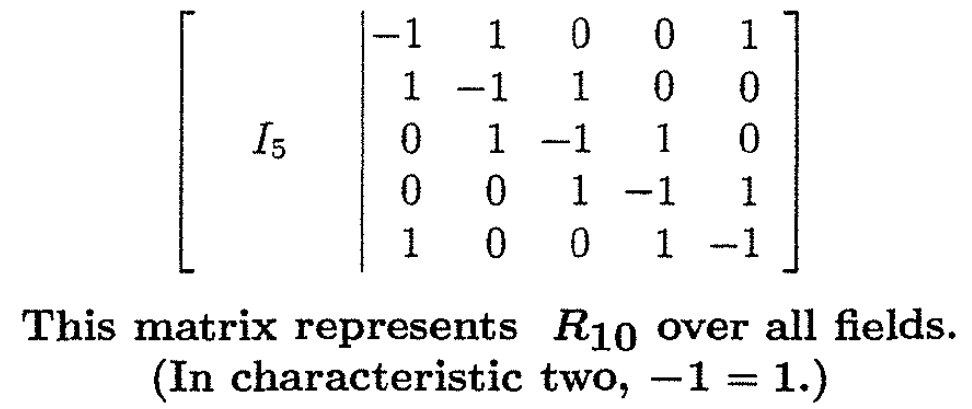
\includegraphics[width=8cm]{Test3/Problem2/R10.png}
    \end{center}\pn
}
\begin{proof}
    As in the previous problem we are going to approach each case.
    
    \begin{itemize}
        \item [$1 \times 1$]
            Any entry is -1, 0 or 1, so its determinat will be -1, 0 or 1.\pn
        \item [$2 \times 2$]
            As we saw before, any column containing only one non-zero entry will result in the determinant of a 
            $1 \times 1$ with a possibly change of sign, and any column with only zeros will result in a determinant
            zero. Then, the only case left is the case with no zero entries.\pn
            
            There is essentially one case, which is
                \begin{align}
                    N =
                        \bordermatrix{
                                &       &       \cr
                                &   1   &  -1   \cr
                                &  -1   &   1  
                        }    
                \end{align}
                
            (given to ones in a column, there is no other column which contains non-zero values in the same rows).
            The determinant of $N$ is 0 and then we have finished this part of the proof.
        
        \item [$3 \times 3$]
            There is no case in cases that include columns from $I_5$. Every column of $I_5$ has at most one $1$ and 
            then, those cases can be reduced to $2 \times 2$ cases, which we have already proved to be totally unimodular.\pn
            
            We would do exhaustive search over all the $\binom{5}{3} \binom{5}{3} = 100$, $3 \times 3$ submatrices, but we won't.
            We will take advantage of the symmetries of the 5 last columns.\pn
            
            Because of the symmetries, we can fix column 6 and any other case will be similar up to permutations.\pn
            
            This has already reduced the space to $\binom{5}{3} \binom{4}{2} = 60$ cases. Which is still quite large.\pn
            
            Now, remember that any case in which we have a column with only one non-zero entry can be reduced to a case
            of a $2 \times 2$ submatrix (up to determinant sign), this gets rid of three possible row choices 
            ($\{1, 3, 4\}, \{2, 3, 4\}, \{3, 4, 5\}$). Wich reduces the space to $\left(\binom{5}{3} - 3\right) \binom{4}{2} = 42$.\pn
            
            We will reduce cases applying this kind of arguments in even more specific subcases. Always think that column 6 is fixed.\pn
            
            \begin{itemize}
                \item[rows 1, 2, 3.]
                    We cannot choose columns 9 or 10 because they will end up with only one non-zero entry.
                    So the only case to check is choosing columns 7 and 8 (along with 6 which is fixed). This
                    submatrix has determinant 1 and then we are done with this subcase.
                \item[rows 1, 2, 4.]
                    We cannot choose column 9 because of the same reason. We cannot choose column 7 or we will have
                    two zeros in row 4. Then we must choose columns 8 and 10. And the resultant submatrix has
                    determinant 0 and then we are done with this subcase.
                \item[rows 1, 2, 5.]
                    We cannot choose columns 8 or 9. We cannot choose columns 7 and 8 together or row 5 will end up with two zeros.\pn
                    The two remaining case is choosing columns 7 and 10. And it is analog to the case when choosing rows 1, 2, 3 reordering rows as
                    5, 1, 2 and columns as 10, 6, 7.
                \item[rows 1, 3, 5.]
                    This subcase is analog to choosing rows 1, 2, 4 up to permutations.
                \item[rows 1, 4, 5.]
                    This subcase is analog to choosing rows 1, 2, 3 up to permutations.
                \item[rows 2, 3, 5.]
                    We cannot choose column 10 or it will have two zeros. We cannot choose columns 7 and 8 together or row 5 will have 
                    two zeros.\pn
                    The two remaining cases are choosing 7 and 9 or 8 and 9. Whose determinats are both 0. And we are done with this case.
            \end{itemize}
            
            In the end we only needed to check the determinant seven cases.
            
        \item [$4 \times 4$]
            Again, we will only check submatrices obtainded from the five last columns. Any other case can be reduced to a $3 \times 3$
            case up to determinant sign.\pn
            
            Te symmetry in the five last columns lets us get rid of any row, it would be the same to delete any of them. So we will not
            take into account the row 5.
            
            Now we only have five cases depending on which columns we choose.
            \begin{itemize}
                \item[columns 6, 7, 8, 9.]
                    The determinant is -1.
                \item[columns 6, 7, 8, 10.]
                    The determinant is 0.
                \item[columns 6, 7, 9, 10.]
                    The determinant is 1.
                \item[columns 6, 8, 9, 10.]
                    The determinant is -1.
                \item[columns 7, 8, 9, 10.]
                    The determinant is 0.
            \end{itemize}
            
             Any other case can be seen as one of these by permuting rows and columns.
        \item [$5 \times 5$]
            Here we have only one interesting case. Choosing all the five last columns. And it has determinant 1.
    \end{itemize}
\end{proof}